\documentclass{article}
\usepackage{CJK} 
\usepackage{graphics}
\usepackage{pgf}
\usepackage{tikz}
\usetikzlibrary{calc,shadows}
\usetikzlibrary{decorations.markings,scopes}
\usetikzlibrary{arrows,snakes,backgrounds,shapes}
\usetikzlibrary{decorations.pathmorphing}
\usepackage{listings}
\renewcommand{\ttdefault}{pcr}
\lstset{
  keywordstyle=\color{blue!70},
  frame=single,
  basicstyle=\ttfamily\bfseries\small,
  commentstyle=\small\color{red},
  rulesepcolor=\color{red!20!green!20!blue!20},
  tabsize=4,
  numbersep=5pt,
  %% backgroundcolor=\color{black!10},
  showspaces=false,
  showtabs=false,
  extendedchars=false,
  escapeinside=``,
  frame=no
}

\newcommand{\blue}{\textcolor{blue}}
\newcommand{\red}{\textcolor{red}}
\newcommand{\purple}{\textcolor{purple}}


\pgfrealjobname{survey}
\begin{document}
  \beginpgfgraphicnamed{figure}
  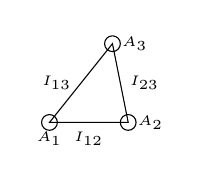
\begin{tikzpicture}
    \draw[] (0,0)--node[midway,below]{\tiny$I_{12}$}(1,0)--node[midway,right]{\tiny$I_{23}$}(.8,1)--node[midway,left]{\tiny$I_{13}$}cycle;
    \draw (0,0) node[below] {\tiny $A_1$} circle (.1);
    \draw (1,0) node[right] {\tiny $A_2$} circle (.1);
    \draw (0.8,1) node[right] {\tiny $A_3$} circle (.1);
  \end{tikzpicture}
  \endpgfgraphicnamed  

\end{document}


